\documentclass[a4paper,
fontsize=11pt,
%headings=small,
oneside,
numbers=noperiodatend,
parskip=half-,
bibliography=totoc,
final
]{scrartcl}

\usepackage[babel]{csquotes}
\usepackage{synttree}
\usepackage{graphicx}
\setkeys{Gin}{width=.4\textwidth} %default pics size

\graphicspath{{./plots/}}
\usepackage[ngerman]{babel}
\usepackage[T1]{fontenc}
%\usepackage{amsmath}
\usepackage[utf8x]{inputenc}
\usepackage [hyphens]{url}
\usepackage{booktabs} 
\usepackage[left=2.4cm,right=2.4cm,top=2.3cm,bottom=2cm,includeheadfoot]{geometry}
\usepackage{eurosym}
\usepackage{multirow}
\usepackage[ngerman]{varioref}
\setcapindent{1em}
\renewcommand{\labelitemi}{--}
\usepackage{paralist}
\usepackage{pdfpages}
\usepackage{lscape}
\usepackage{float}
\usepackage{acronym}
\usepackage{eurosym}
\usepackage{longtable,lscape}
\usepackage{mathpazo}
\usepackage[normalem]{ulem} %emphasize weiterhin kursiv
\usepackage[flushmargin,ragged]{footmisc} % left align footnote
\usepackage{ccicons} 
\setcapindent{0pt} % no indentation in captions

\usepackage{subcaption}


%%%% fancy LIBREAS URL color 
\usepackage{xcolor}
\definecolor{libreas}{RGB}{112,0,0}

\usepackage{listings}

\urlstyle{same}  % don't use monospace font for urls

\usepackage[fleqn]{amsmath}

%adjust fontsize for part

\usepackage{sectsty}
\partfont{\large}

%Das BibTeX-Zeichen mit \BibTeX setzen:
\def\symbol#1{\char #1\relax}
\def\bsl{{\tt\symbol{'134}}}
\def\BibTeX{{\rm B\kern-.05em{\sc i\kern-.025em b}\kern-.08em
    T\kern-.1667em\lower.7ex\hbox{E}\kern-.125emX}}

\usepackage{fancyhdr}
\fancyhf{}
\pagestyle{fancyplain}
\fancyhead[R]{\thepage}

% make sure bookmarks are created eventough sections are not numbered!
% uncommend if sections are numbered (bookmarks created by default)
\makeatletter
\renewcommand\@seccntformat[1]{}
\makeatother

% typo setup
\clubpenalty = 10000
\widowpenalty = 10000
\displaywidowpenalty = 10000

\usepackage{hyperxmp}
\usepackage[colorlinks, linkcolor=black,citecolor=black, urlcolor=libreas,
breaklinks= true,bookmarks=true,bookmarksopen=true]{hyperref}
\usepackage{breakurl}

%meta
%meta

\fancyhead[L]{M. Platon\\ %author
LIBREAS. Library Ideas, 38 (2020). % journal, issue, volume.
\href{https://doi.org/10.18452/23472}{\color{black}https://doi.org/10.18452/23472}
{}} % doi 
\fancyhead[R]{\thepage} %page number
\fancyfoot[L] {\ccLogo \ccAttribution\ \href{https://creativecommons.org/licenses/by/4.0/}{\color{black}Creative Commons BY 4.0}}  %licence
\fancyfoot[R] {ISSN: 1860-7950}

\title{\LARGE{Farewell Gundula! Obituary to our library plant!}}% title
\author{Marjorie Platon} % author

\setcounter{page}{1}

\hypersetup{%
      pdftitle={Farewell Gundula! Obituary to our library plant!},
      pdfauthor={Marjorie Platon},
      pdfcopyright={CC BY 4.0 International},
      pdfsubject={LIBREAS. Library Ideas, 38 (2020).},
      pdfkeywords={Bibliothek, Pflanze, Nachruf, library, plant, obituary},
      pdflicenseurl={https://creativecommons.org/licenses/by/4.0/},
      pdfcontacturl={http://libreas.eu},
      baseurl={http://libreas.eu},
      pdflang={en},
      pdfmetalang={en}
     }



\date{}
\begin{document}

\maketitle
\thispagestyle{fancyplain} 

%abstracts

%body

\begin{figure}[h!]
\centering
\begin{subfigure}{.5\textwidth}
  \centering
  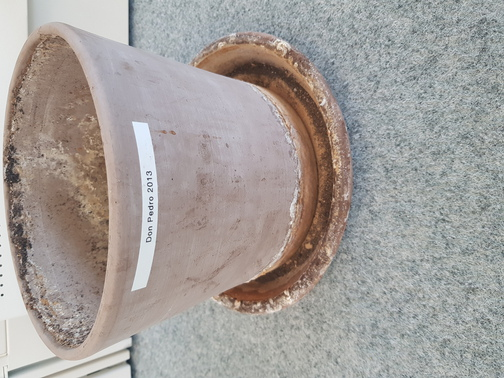
\includegraphics[angle=270,width=.7\linewidth]{img/20200731-080331.jpg}
\end{subfigure}%
\begin{subfigure}{.5\textwidth}
  \centering
  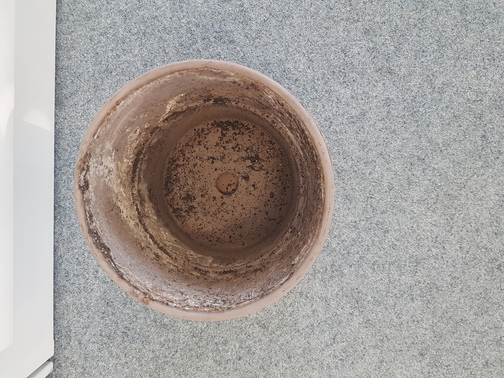
\includegraphics[angle=270,width=.7\linewidth]{img/20200731-080339.jpg}
\end{subfigure}
\end{figure}

%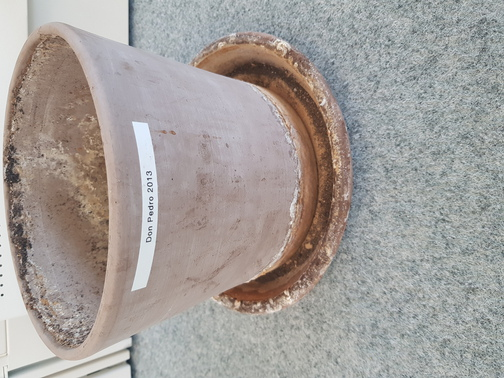
\includegraphics[angle=270]{img/20200731-080331.jpg}

%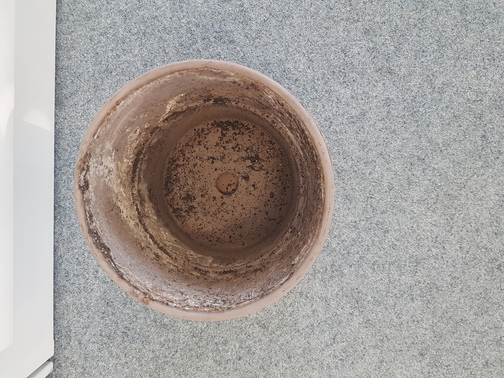
\includegraphics[angle=270]{img/20200731-080339.jpg}

Adopted in 2013 at the EPFL library following a \enquote{librarian
Pedro-to-librarian Marjorie} donation, Gundula passed away in June 2020
at the Rolex Learning Center.

The office shutdown combined with the heatwave got the better of you.
Life is hard for a papyrus if it does not have water. The windows of the
building are dangerous. Gundula resisted well, but without her librarian
to water her, she withered and then dried up.

When she died, her librarian in charge wanted her to be buried in front
of the library staff entrance so that she could rest where she lived for
7 years.

Farewell Gundula, your long green stems and your parasol leaves will be
missed.

%autor
\begin{center}\rule{0.5\linewidth}{0.5pt}\end{center}

\textbf{Marjorie Platon}: Information specialist at the EPFL Library for
the past 10 years, Marjorie works for the ``service au public''. She
manages the schedules of the counter staff. She is also in charge of the
Student Assistants. Her professional hobbies are standards and
copyright. To keep pace, she likes to taste the typical dishes brought
by her colleagues.

\end{document}
